\documentclass{article}
\usepackage[utf8]{inputenc}
\usepackage{caption}
\usepackage[margin=1in]{geometry}
\usepackage{graphicx}
\usepackage{pdfpages}
\usepackage{float}
\pdfminorversion=7

\begin{document}
\begin{titlepage}


\centering
\vspace*{2cm}
{\Huge User Interface Design Document\par}
\vspace{.25cm}
{\LARGE Course Evaluation System\par}
\vspace{1cm}
{\Large Team EVAL\par}
\vspace{.2cm}
{\Large Jovon Craig, Sam Elliott, Robert Judkins, and Stanley Small\par}
\vspace{1cm}
{\Large Client: Dr. Harlan Onsrud\par}
\vspace{1cm}
{\Large November 30, 2018\par}
\vspace{11cm}

University of Maine - Fall of 2018 - COS 397

Instructor: Professor Terry Yoo

\end{titlepage}

\newpage

\begin{center}
{
\includegraphics[scale=.2]{images/team_logo.png}} \\ 	\bigskip
{\LARGE Course Evaluation System } \\ \medskip
{\large User Interface Design Document } \\ \medskip
\end{center}

\tableofcontents

\newpage

\section{Introduction}
 

\subsection{Purpose of This Document}

This user interface design document is an overview of the graphics and layouts shown to the users of our course evaluation system. The first section, the user interface standards, describes the general features of the graphics, such as layouts and components, that are common to all screens in the interface. The second section, the user interface walkthrough, includes a ``navigation diagram'' of the order in which screens appear, as well as complete wireframes of each screen. The docuement's third section gives the data items typically entered in the user interface and how they are formatted.

This document is intended for the development team, the product client, Dr. Harlan Onsrud, and potential users of the system. Team EVAL needs this document to properly implement the user interface in code. Dr. Onsrud also needs it to verify that the program's appearance looks appropriate for universities. Lastly, the document helps the software's users in that it serves as a guide for how to use the software.


\subsection{References}

Craig, J., Elliott, S., Judkins, R., \& Small, S. 29 October 2018. \textit{System Requirements Specification.}
\vspace{3mm}\newline
Craig, J., Elliott, S., Judkins, R., \& Small, S. 16 November 2018. \textit{System Design Document.}
\vspace{3mm}\newline
Onsrud, H. ``Example Question Selection Form.'' See Appendix D.
\vspace{3mm}\newline
Onsrud, H. ''Report for Professor: Roy Turner'' See Appendix E.

\section{User Interface Standards}

The interface of the course evaluation system is standardized; several components are present in multiple screens. Figure 1, shown on the next page, is the overall screen layout of our course evaluation system. It shows the general areas and components of the screens in the user interface. Not all screens follow the exact overall layout.

\newpage

\begin{center}
\captionof{figure}{Overall layout of a screen in the UI}
\vspace{3mm}
{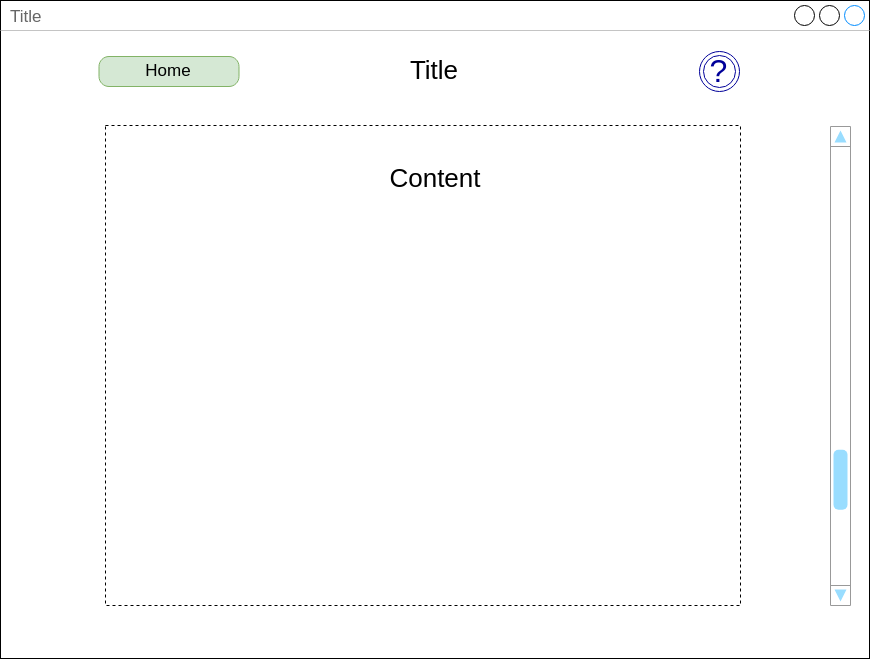
\includegraphics[width=6.5in]{images/overall_layout.png}}
\vspace{2mm}
\end{center}

For ease of use, the team made the designs simple for each screen. On the top-right corner, there is the team EVAL logo and the name of the program. The top-right corner includes navigation buttons, typically a a ``Home'' button, which returns the user to the home screen, and the ``Log Out'' button, which takes the user to the log-in screen. The ``content'' is located below the top elements and contains data entry fields, evaluation results, and the like. In sections that may be look complicated, a help pop-up will appear when the mouse is over the question mark icon. Most screens also have a scroll bar on the right side if the information on a page cannot all fit in the web browser.

\newpage

\section{User Interface Walkthrough}

This section goes into more detail about the screens in the user interface and how an administrator or instructor navigates through them. Figure 2 shows the navigation diagram, which shows the paths that a user can take through the system's interface. The diagram also includes the names for all the screens in the UI. 

\begin{center}
\captionof{figure}{Navigation diagram of the user interface}
\vspace{3mm}
{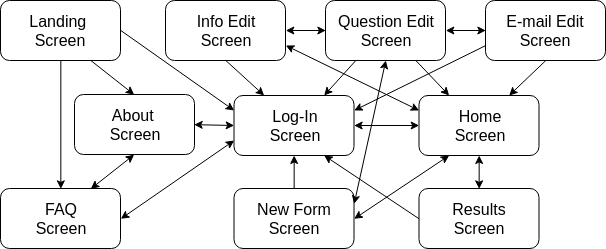
\includegraphics[width=6.5in]{images/navigation_diagram.png}}
\vspace{2mm}
\end{center} 

The first screen that the user sees upon starting up the system is the \textbf{Landing Screen}. Next, the user can view the \textbf{About Screen}, \textbf{FAQ Screen}, or  \textbf{Log-In Screen} and switch between the three. After entering a correct username and password on the log-in screen, the \textbf{Home Screen} appears. The user can then call up the \textbf{Info Edit Screen}, \textbf{New Form Screen}, or \textbf{Results Screen} from the home page or return to the about or FAQ screens. You must go to the new form screen to create a survey or the info edit screen to modify a survey. Next, the user proceeds to the \textbf{Question Edit Screen} and then the \textbf{E-mail Edit Screen}. The log-in screen and home screen can be accessed from any other screen except the landing, about, and FAQ screens.

The next set of figures, Figures 3 to 12, consist of the wireframes for each screen in the evaluation system. These diagrams communicate the areas, menus, and buttons that are unique to a certain screen and what they do.

\newpage
\newgeometry{left=1in, right=1in, top=2cm, bottom=2cm}

\begin{center}
\begin{figure}[H]
    \centering
    \caption{Landing screen}
    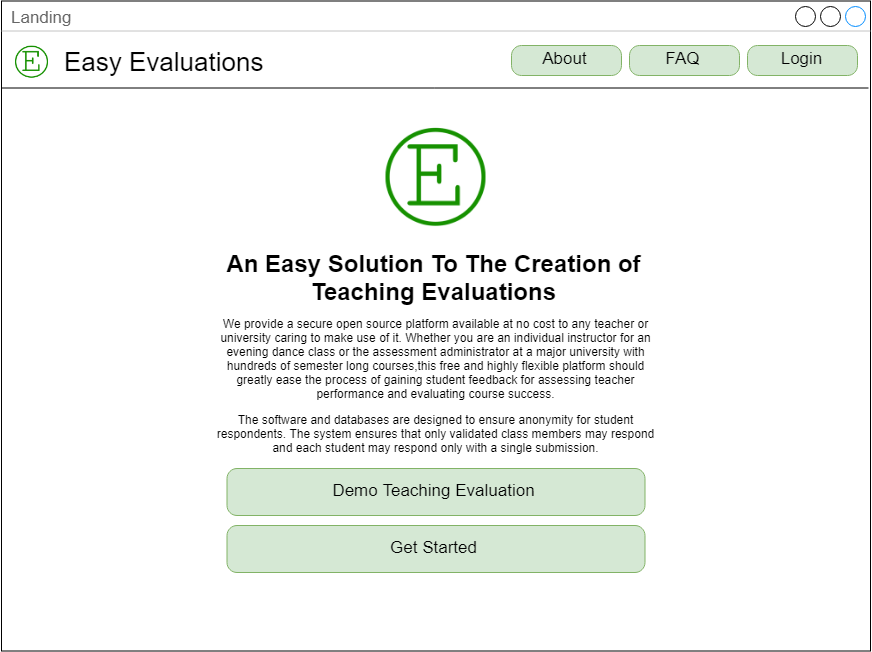
\includegraphics[width=6.5in]{images/landing_screen.png}
\end{figure}
\end{center}

This is the first screen a user would see when entering the website. A user could click on the ``Demo Teaching Evaluation'' button, which would link to an informative video. Clicking ``Get Started'' would lead them to an account creation screen. Alternatively they could click ``About'', ``FAQ'', or ``Sign In'' to enter the corresponding screens.

\newpage

\begin{center}
\begin{figure}[H]
    \centering
    \caption{Log-in screen}
    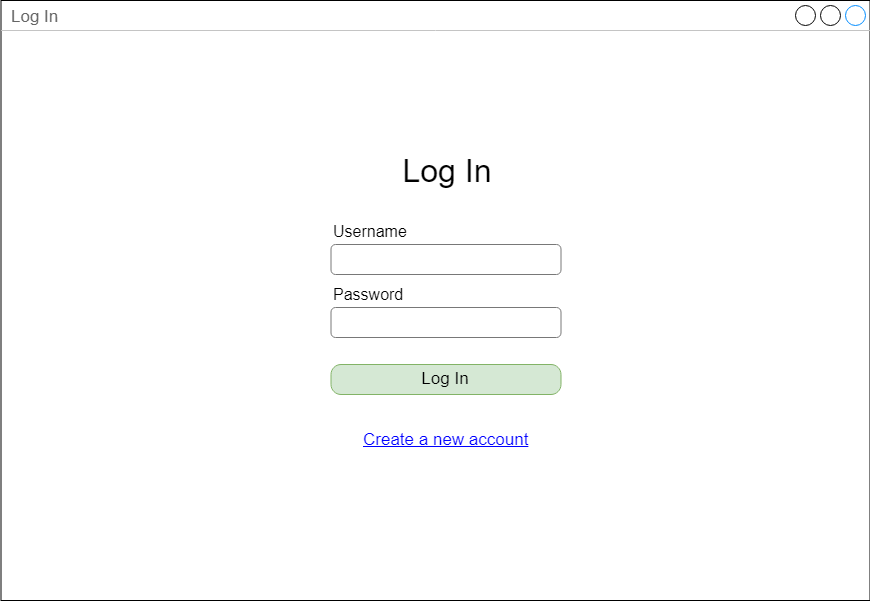
\includegraphics[width=6.5in]{images/login_screen.png}
\end{figure}
\end{center}

A user would enter a valid username and password to log in. Clicking ``Log In'' advances the user to the selection screen. The ``About'', ``FAQ'', and ``Sign In'' buttons would take you to their respective pages.

\newpage

\begin{center}
\begin{figure}[H]
    \centering
    \caption{FAQ Screen}
    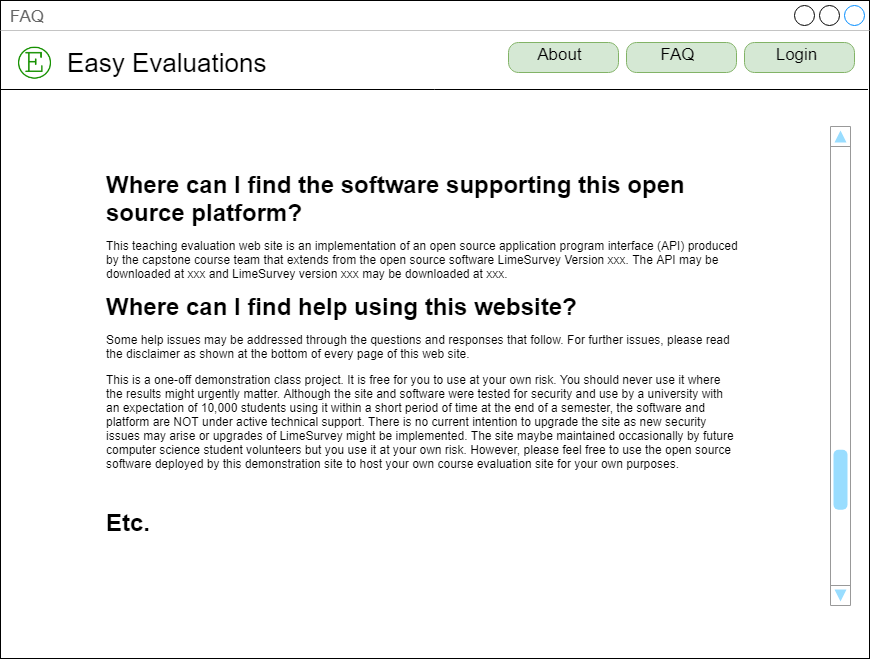
\includegraphics[width=6.5in]{images/faq_screen.png}
\end{figure}
\end{center}

This screen details frequently asked questions that a user may have and their answers. The ``About'', ``FAQ'', and ``Sign In'' buttons would take you to their respective pages.

\newpage

\begin{center}
\begin{figure}[H]
    \centering
    \caption{About screen}
    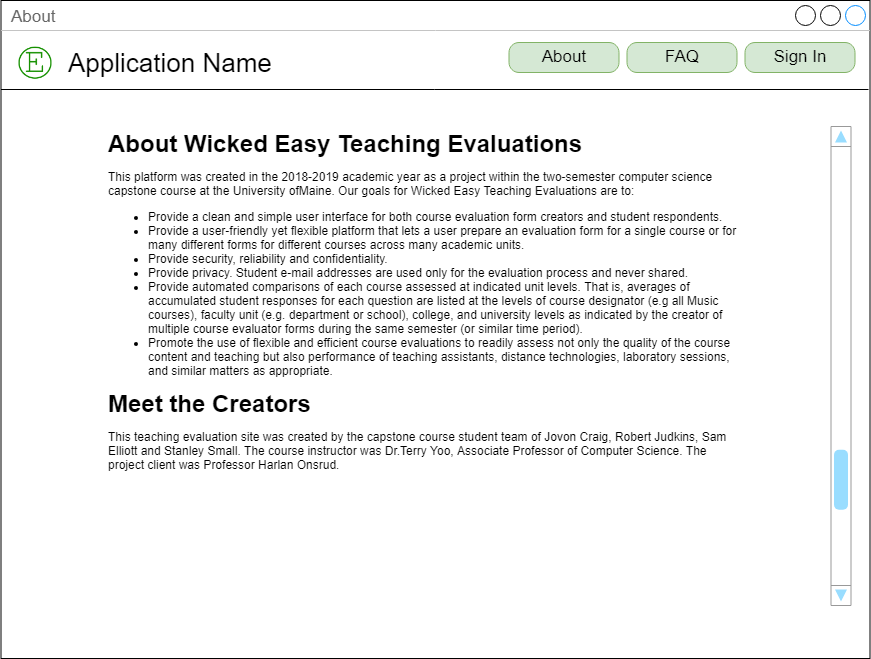
\includegraphics[width=6.5in]{images/about_screen.png}
\end{figure}
\end{center}

This screen gives details about the product and its purpose. It also credits the creators, as well as the client for whom the product was made. The ``About'', ``FAQ'', and ``Sign In'' buttons would take you to their respective pages.

\newpage

\begin{center}
\begin{figure}[H]
    \centering
    \caption{Home screen}
    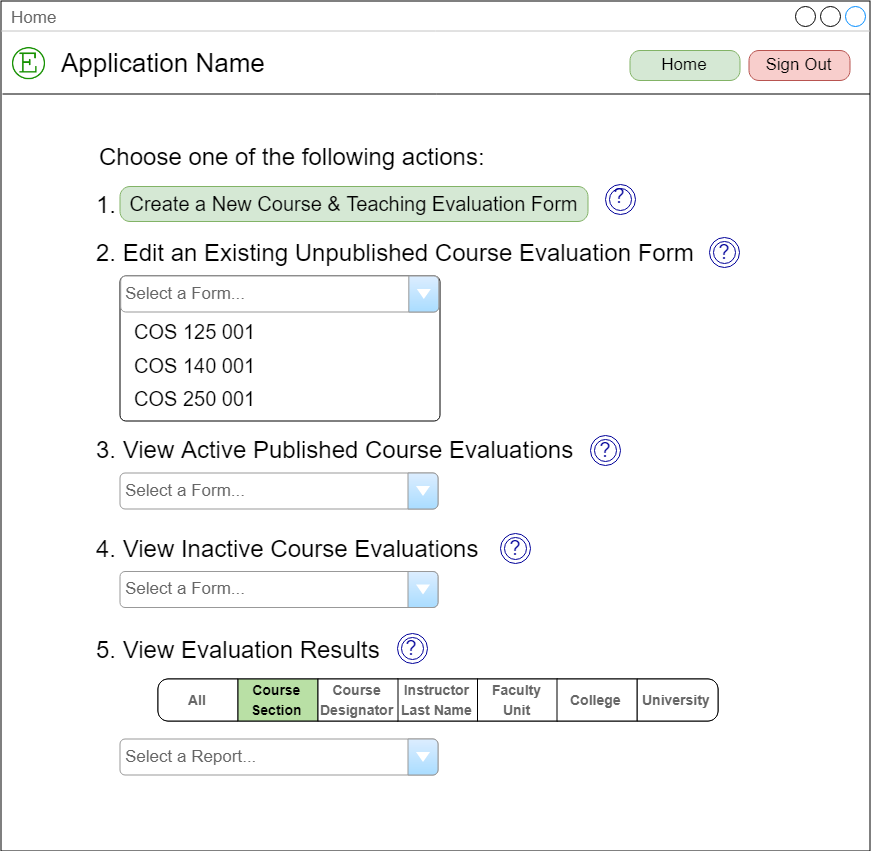
\includegraphics[width=6.5in]{images/home_screen.png}
\end{figure}
\end{center}

This is the main screen a user would see after logging in. Users can choose to (1) create a new evaluation form, which will redirect them to the new form screen. They can (2) select a course which has been saved but unfinished and unpublished, redirecting them to the info edit screen. They can (3) select a course that has already been published but not completed, taking them to the edit screen where information is displayed but not editable. Also, they can  (4) select a course that has been published and completed, taking them to the edit screen where information is displayed but not editable. Finally, they can (5) select to view evaluation results. One must choose a category type with the menu bar and a category name with the drop-down menu, making the results page appear.

\newpage

\begin{center}
\begin{figure}[H]
    \centering
    \caption{New form screen}
    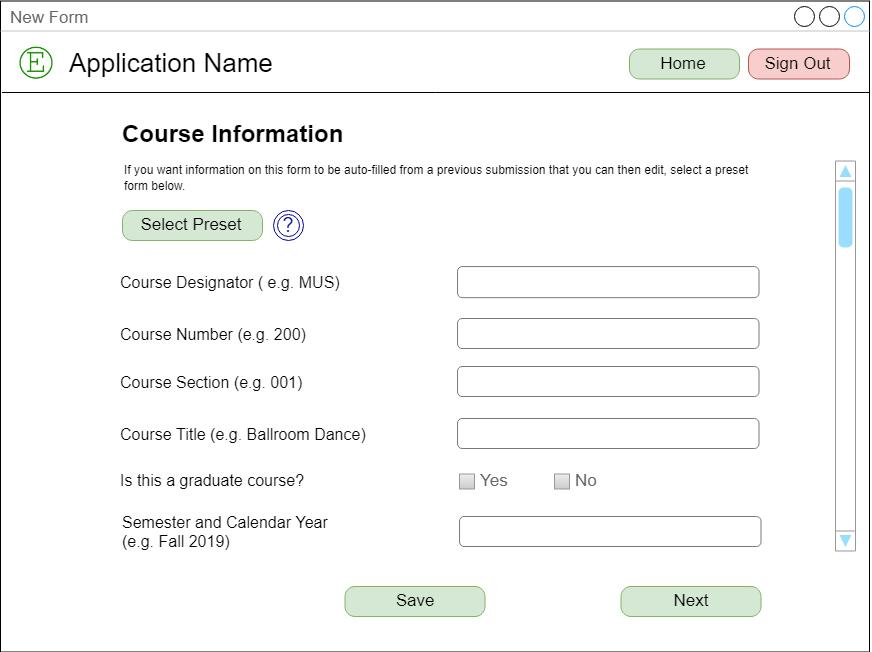
\includegraphics[width=6.5in]{images/create_screen.png}
\end{figure}
\end{center}

This is the page users would see if they decided to create a new evaluation form. This page asks the user to fill out the general information of the course for which the evaluation form applies. Alternatively, the user can select a previously created preset rather than starting from scratch. See Appendix D page 1 for a full example of all fields that will be shown.  The ''Save'' button will save the currently entered information. The ''Next'' button takes the user to the question edit screen.

\newpage

\begin{center}
\begin{figure}[H]
    \centering
    \caption{Info edit screen}
    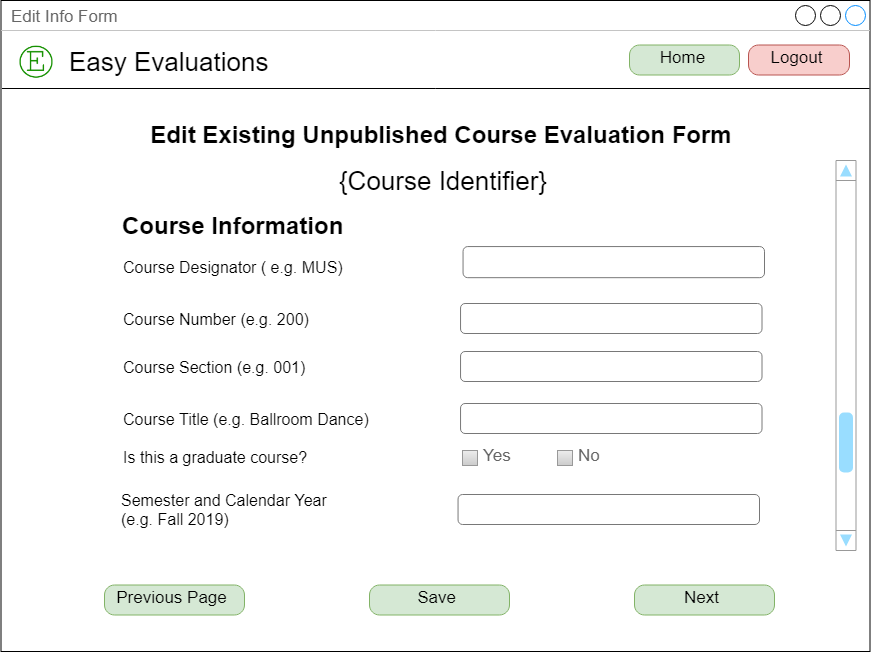
\includegraphics[width=6.5in]{images/edit_info_screen.png}
\end{figure}
\end{center}

Similar to the new form screen, a user would be redirected to this screen when choosing to edit an evaluation previously created but left unfinished or unpublished. The page allows users to view and edit the information of an existing unpublished evaluation form.  The ``Previous'' button redirects users to the home page, the ``Next'' button redirects them to the question edit screen, and the ``Save'' button saves the entered information. See Appendix D for a full example of available questions to choose from.

\newpage

\begin{center}
\begin{figure}[H]
    \centering
    \caption{Question edit screen}
    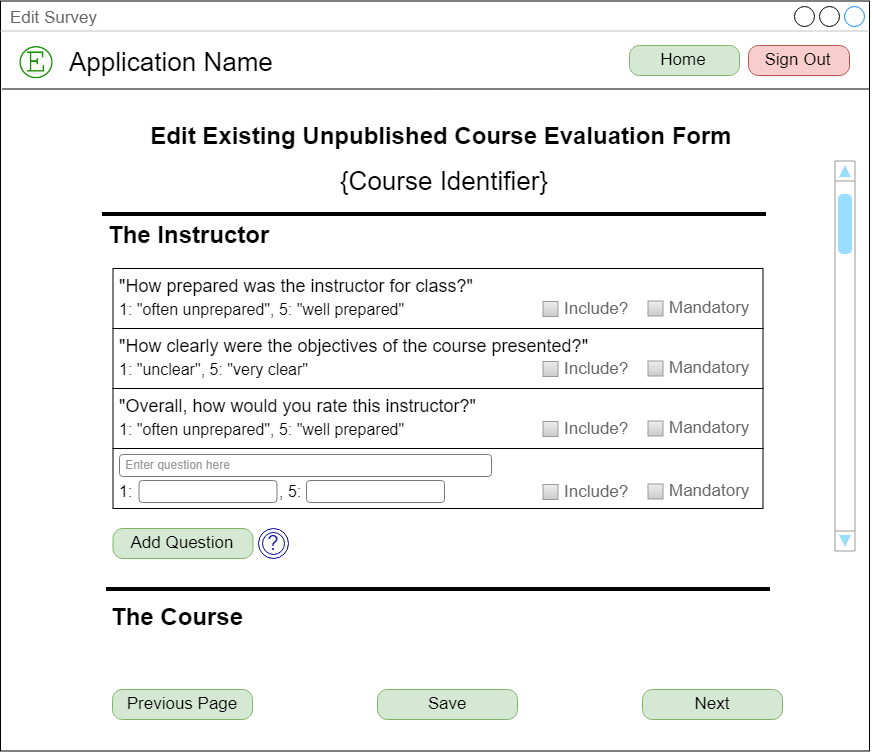
\includegraphics[width=6.5in]{images/questions_screen.png}
\end{figure}
\end{center}

This is the second page a user would see when creating a course evaluation. You are redirected here after pressing the next button from the new form page or info edit page.  The ``Previous'' button redirects the user to the question edit screen, the ``Next'' button goes to the e-mail edit screen, and the ``Save'' button saves the entered data. The page lists several generic questions that may be asked in a evaluation form. It also asks if the instructor would like to include a certain question and whether it should be mandatory. Users can also add custom questions at each section. See Appendix D for a full example.

\newpage

\begin{center}
\begin{figure}[H]
    \centering
    \caption{E-mail edit screen}
    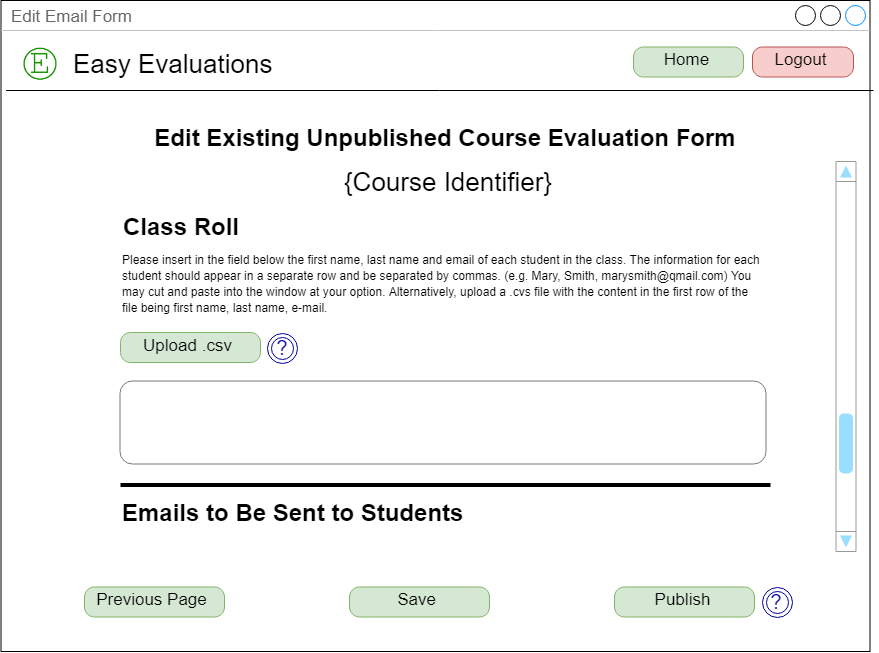
\includegraphics[width=6.5in]{images/emails_screen.png}
\end{figure}
\end{center}

This is the final page a user would see when creating a new course evaluation. They will be redirected here when the ``Next'' button is pressed on the question edit Screen. It asks the instructor to include a list of students taking the course, to review a generic e-mail that would be sent to students, and to review a reminder e-mail that could be sent after a certain period of time. See Appendix D for a full example.

\newpage

\begin{center}
\begin{figure}[H]
    \centering
    \caption{Results screen}
    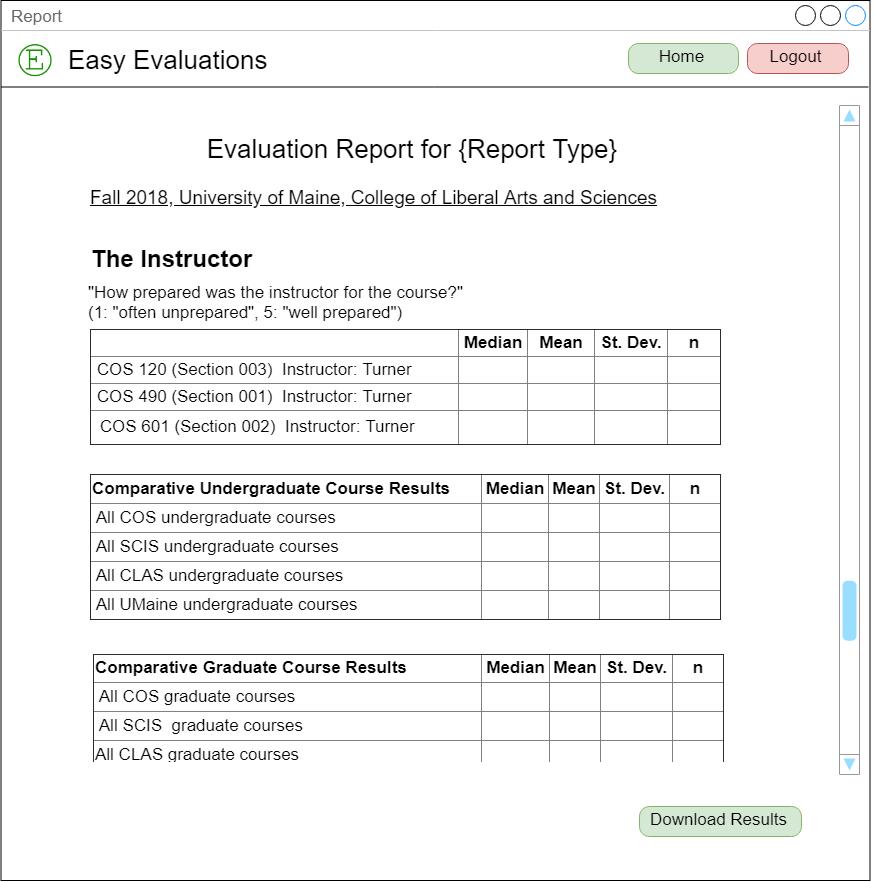
\includegraphics[width=6.5in]{images/report_screen.png}
\end{figure}
\end{center}

This page is where a user would view results of their evaluations based on the category selected on the home screen.  The responses are organized by each question in the evaluation and displays different tables for undergraduate courses and graduate courses. It includes the median, mean, standard deviation, and number of answers for each question along with question statistics for the classes in the selected category. The results can also be downloaded and exported as a .csv file by clicking the ``Download Results'' button. See Appendix D for a full example of an instructor report.

\newpage

\section{Data Validation}

Table 1 lists the data items in the user interface of the evaluation system. A data item is an input that a user enters into the system and has a specified format. Many of the items listed are for editing a course evalution form.

\begin{center}
\captionof{table}{Data item specification}
\scalebox{.92}{
\begin{tabular}{|p{4.4cm}|p{2.4cm}|p{1.5cm}|p{4cm}|p{3cm}|} 
\hline
\textbf{Label} & \textbf{Screen(s)} & \textbf{Data Type} & \textbf{Format} & \textbf{Limit(s)} \\
\hline
Username & Log in & String & username@gmail.com & N/A \\ 
\hline
Password & Log in & String & N/A & N/A \\ 
\hline
Course designator & New form, info edit & String & N/A & 50 characters long\\ 
\hline
Course number & New form, info edit & String & N/A & 50 characters long\\ 
\hline
Course section & New form, info edit & String & N/A & 50 characters long\\ 
\hline
Course title & New form, info edit & String & N/A & 50 characters long\\ 
\hline
Graduate course & New form, info edit & Boolean & N/A & 50 characters long\\ 
\hline
Semester and year & New form, info edit & String & N/A & 50 characters long\\ 
\hline
Faculty unit & New form, info edit & String & N/A & 50 characters long\\ 
\hline
Department & New form, info edit & String & N/A & 50 characters long\\ 
\hline
University & New form, info edit & String & N/A & 50 characters long\\ 
\hline
Instructor first name & New form, info edit & String & N/A & 50 characters long\\ 
\hline
Instructor last name & New form, info edit & String & N/A & 50 characters long\\ 
\hline
Instructor e-mail & New form, info edit & String & N/A & 50 characters long\\ 
\hline
Instructor phone & New form, info edit & String & N/A & 50 characters long\\ 
\hline
Course evaluation administrator & New form, info edit & String & N/A & 50 characters long\\ 
\hline
Evaluation administrator e-mail & New form, info edit & String & N/A & 50 characters long\\ 
\hline
Starting assessment date & New form, info edit & String & mm/dd/yy & 50 characters long\\ 
\hline
Mailing time & New form, info edit & String & hh:mm:ss & 50 characters long\\ 
\hline
Closing assessment date & New form, info edit & String & N/A & 50 characters long\\ 
\hline
Added questions & Question edit & Strings & N/A & 150 characters long\\ 
\hline
1 score label & Question edit & String & N/A & 50 characters long\\
\hline
5 score label & Question edit & String & N/A & 50 characters long\\
\hline
``Include?'' checkboxes & Question edit & Boolean & N/A & N/A \\ 
\hline
``Mandatory'' checkboxes & Question edit & Boolean & N/A & N/A \\ 
\hline
Class roll & E-mail edit & String & Comma-separated lines: \newline ``first name, last name, e-mail address'' & N/A \\ 
\hline
Initial e-mail to students & E-mail edit & String & N/A & N/A \\ 
\hline
Reminder e-mail & E-mail edit & String & N/A & N/A\\ 
\hline
Final confirmation e-mail & E-mail edit & String & N/A & N/A\\ 
\hline
\end{tabular}
}
\end{center}

\appendix
\newgeometry{left=1in, right=1in, top=1in, bottom=1in}

\newpage
\section{Agreement Between Customer and Contractor}
This page shows that all members of Team EVAL and the client, Harlan Onsrud, have agreed on all the information in the user interface design document. By signing this document, Team EVAL and Dr. Onsrud approve all of the designs for each screen in the interface, as well as how to navigate the interface.

The team will follow a process in the case that the design document is changed after we sign it. First, the team will write a rough draft of the changes to be made to the document. Second, all team members and Harlan Onsrud will sign the document agreeing to the changes. Finally, the team will make the changes to the final copy of the document.

\vspace{.7in}
\noindent
\begin{tabular}{ p{5cm} p{5cm} p{5cm} } 
\textbf{\textit{Name}} & \textbf{\textit{Signature}} & \textbf{\textit{Date}} \\[.5cm]
\textbf{Jovon Craig} & $\rule{5cm}{.1mm}$ & $\rule{5cm}{.1mm}$\\[.5cm]
\textbf{Sam Elliott} & $\rule{5cm}{.1mm}$ & $\rule{5cm}{.1mm}$\\[.5cm]
\textbf{Robert Judkins} & $\rule{5cm}{.1mm}$ & $\rule{5cm}{.1mm}$\\[.5cm]
\textbf{Stanley Small} & $\rule{5cm}{.1mm}$ & $\rule{5cm}{.1mm}$\\[.5cm]
\textbf{Harlan Onsrud} & $\rule{5cm}{.1mm}$ & $\rule{5cm}{.1mm}$\\[.5cm]
Customer Comments: & \multicolumn{2}{ l }{ $\rule{10.45cm}{.1mm}$ }\\[.5cm]
\multicolumn{3}{ l }{ $\rule{15.9cm}{.1mm}$ }\\[.5cm]
\end{tabular}

\newpage
\section{Team Review Sign-off}

This page shows that all members of Team EVAL have reviewed the user interface design document and agreed on its content. By signing this document, the team members agree that all information about the evaluation system's UI is accurate, and there is nothing in the document that is a source of contention.

\vspace{.7in}
\noindent
\begin{tabular}{ p{5cm} p{5cm} p{5cm} } 
\textbf{\textit{Name}} & \textbf{\textit{Signature}} & \textbf{\textit{Date}} \\[.5cm]
\textbf{Jovon Craig} & $\rule{5cm}{.1mm}$ & $\rule{5cm}{.1mm}$\\[.5cm]
Comments: & \multicolumn{2}{ l }{ $\rule{10.45cm}{.1mm}$ }\\[.5cm]
\multicolumn{3}{ l }{ $\rule{15.9cm}{.1mm}$ }\\[.5cm]
\textbf{Sam Elliott} & $\rule{5cm}{.1mm}$ & $\rule{5cm}{.1mm}$\\[.5cm]
Comments: & \multicolumn{2}{ l }{ $\rule{10.45cm}{.1mm}$ }\\[.5cm]
\multicolumn{3}{ l }{ $\rule{15.9cm}{.1mm}$ }\\[.5cm]
\textbf{Robert Judkins} & $\rule{5cm}{.1mm}$ & $\rule{5cm}{.1mm}$\\[.5cm]
Comments: & \multicolumn{2}{ l }{ $\rule{10.45cm}{.1mm}$ }\\[.5cm]
\multicolumn{3}{ l }{ $\rule{15.9cm}{.1mm}$ }\\[.5cm]
\textbf{Stanley Small} & $\rule{5cm}{.1mm}$ & $\rule{5cm}{.1mm}$\\[.5cm]
Comments: & \multicolumn{2}{ l }{ $\rule{10.45cm}{.1mm}$ }\\[.5cm]
\multicolumn{3}{ l }{ $\rule{15.9cm}{.1mm}$ }\\[.5cm]
\end{tabular}


\newpage
\section{Document Contributions}

Stanley Small contributed to the discussion of the UI design and helped make revisions to the client's request. He also provided some formatting changes to the document. Stan contributed approximately 10 percent of the document.

Jovon Craig wrote the purpose of the document, the user interface standards section, the description of the UI navigation, the first three columns of the data item table, and Appendix C. He created the overall layout diagram, navigation diagram, and many of the individual screen layouts. He revised several screen layouts and parts of the document. Jovon contributed about 35 percent of the document.

Sam Elliott revised all of the individual screen layouts and their descriptions, and he added several new screens. He also wrote the last two columns in the data item table and revised the summaries of each wireframe. Sam contributed about 35 percent of the document.

Robert Judkins converted the UIDD template to the LaTeX format and placed it in our document. He initially wrote the descriptions under each wireframe picture of the UI. He also added the references and appendices A, B, and D. Robert contributed about 20 percent of the document.

\newpage

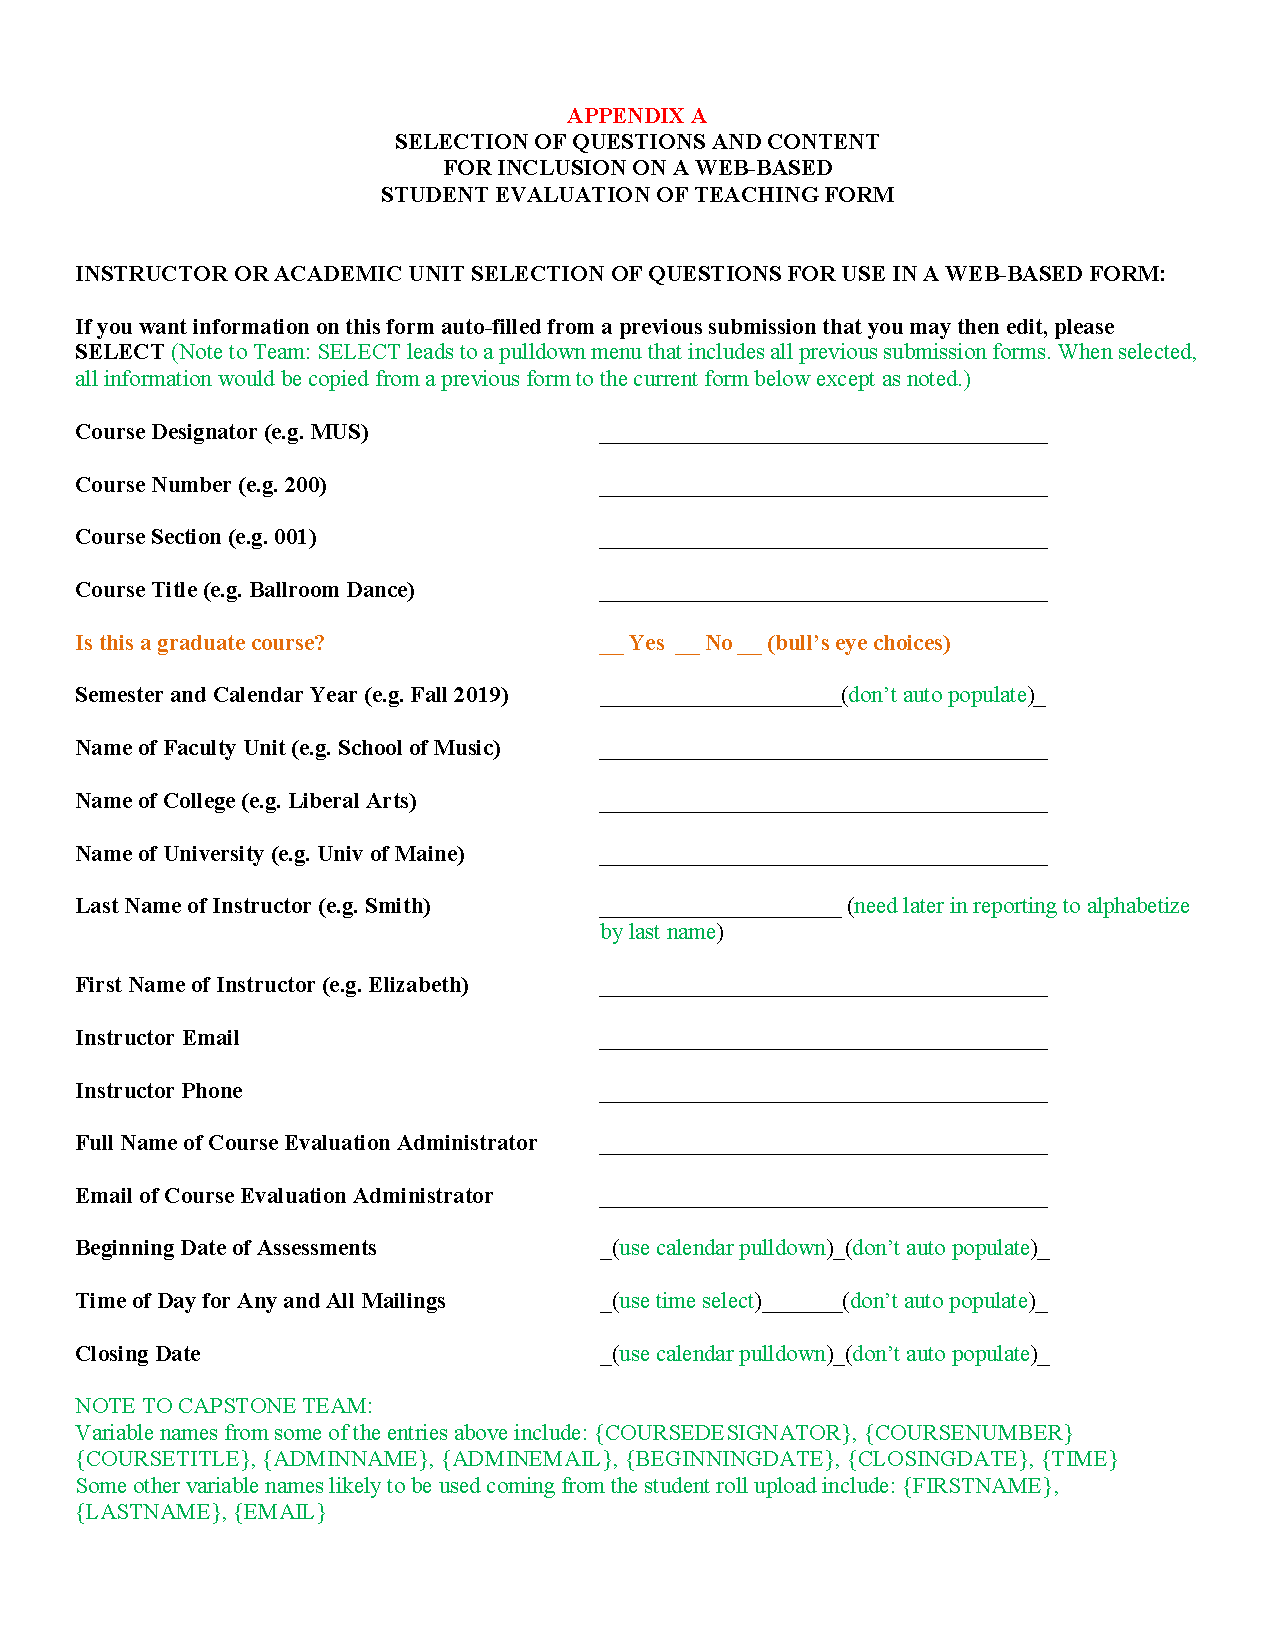
\includepdf[scale=0.85,pages=1,pagecommand=\section{Example Question Selection Form}]{images/question_appendix.pdf}
\includepdf[scale=0.85,pages=2-]{images/question_appendix.pdf}

\newpage

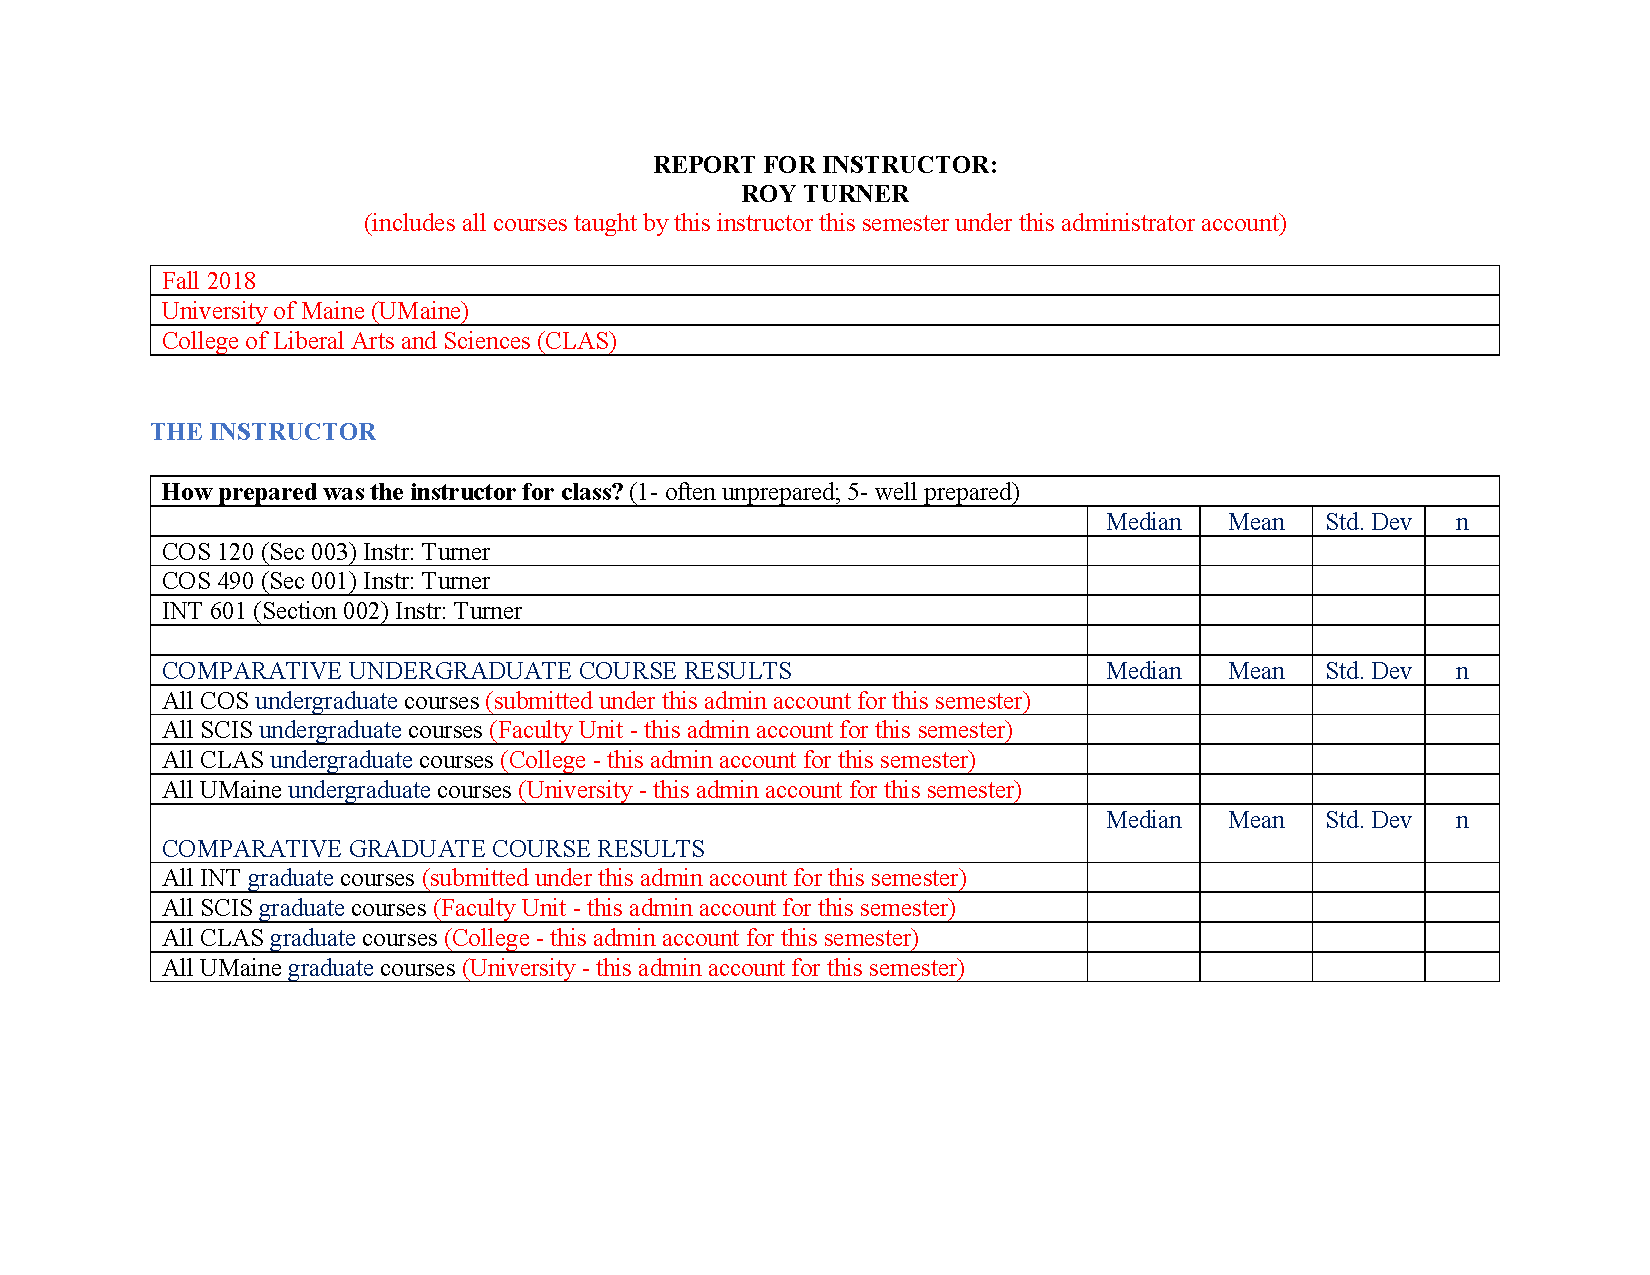
\includepdf[scale=0.92,pages=1,pagecommand=\section{Example Results Display}]{images/results_appendix.pdf}
\includepdf[scale=0.92,pages=2-]{images/results_appendix.pdf}
\end{document}
